
\begin{figure*}[t!]
  \begin{minipage}{.45\textwidth}
      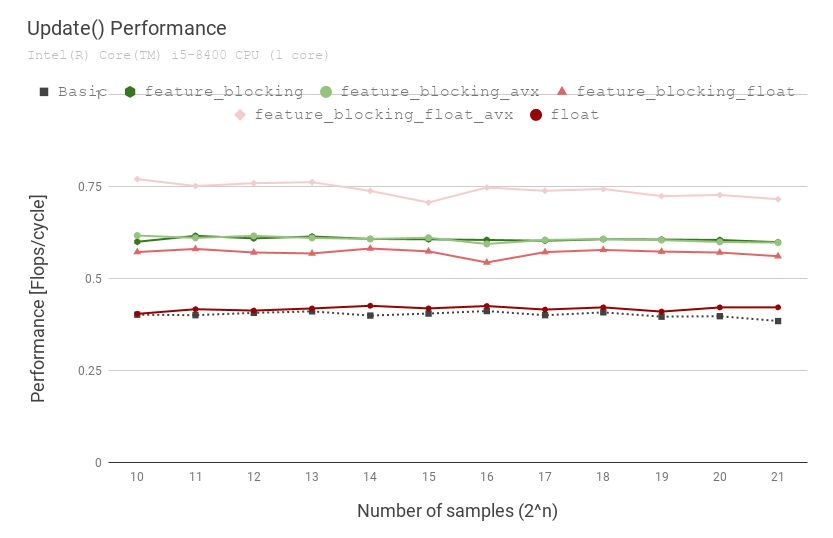
\includegraphics[width=1.0\textwidth]{fig/update.png}
      \caption{Performance of update().}
      \label{fig:update}
      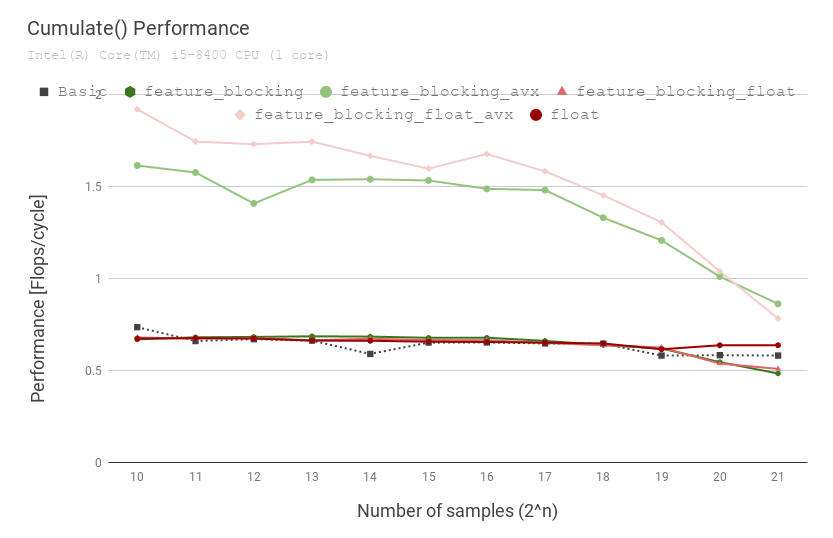
\includegraphics[width=1.0\textwidth]{fig/cumulate.png}
      \caption{Performance of cumulate().}
      \label{fig:cumulate}
  \end{minipage} \quad \quad
  \begin{minipage}{.45\textwidth}
      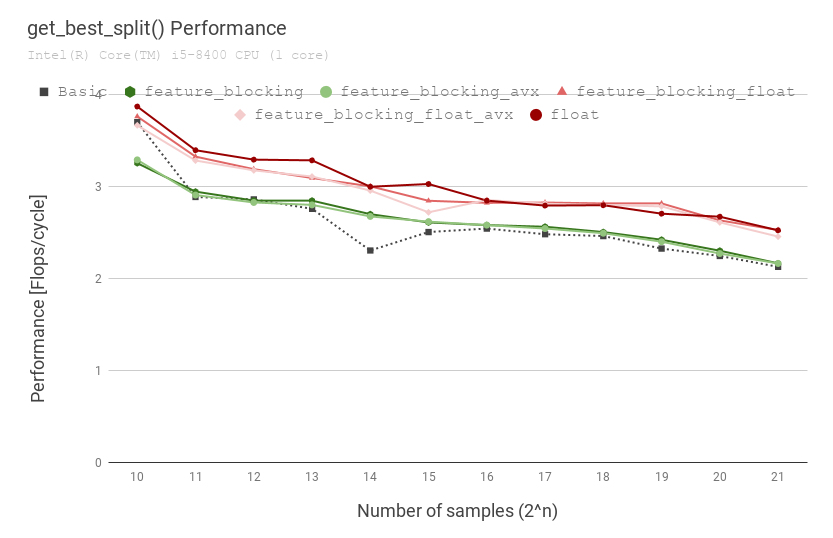
\includegraphics[width=1.0\textwidth]{fig/gbs.png}
      \caption{Performance of get\_best\_splits().}
      \label{fig:gbs}
      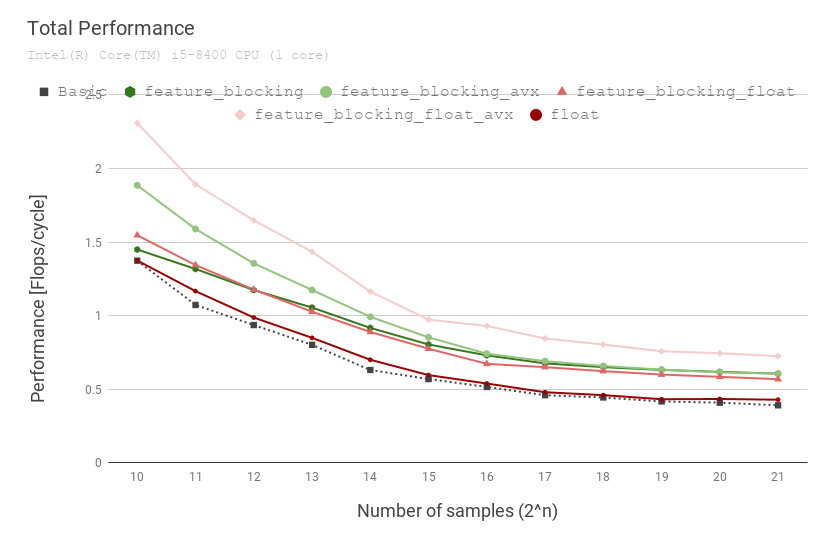
\includegraphics[width=1.0\textwidth]{fig/total.png}
      \caption{Performance of all three functions combined.}
      \label{fig:all}
  \end{minipage}
\end{figure*}
 
\mypar{Experimental setup} We ran our experiments on Intel(R) Core(TM) i5-8400 CPU @ 2.80GHz (Coffee Lake). The machine has L1 cache size of 32KB, L2 cache size of 256KB, and L3 cache size of 9216KB. Our experiments were run on Ubuntu 18.04 and compiled with gcc-7.3.0. We ran all our non-avx experiments with -O3 flag and avx experiments with -O3 -mfma -mavx flags.

We used the MSLR-WEB30K dataset from Microsoft Learning to Rank datasets\footnote{https://www.microsoft.com/en-us/research/project/mslr/}.
In order to compare the performance on different sizes of input, we cut the datasets to have sample numbers varying from $2^{10}$ to $2^{21}$. For each run, we set the number of trees to 10, maximum number of bins to 256, maximum depth to 9.


\mypar{Results}
Figures \ref{fig:update} to \ref{fig:all} show the experimental results of our proposed methods. The baseline method is always displayed in black, and the optimizations in different color gradients. We built our optimizations on top of each other to show that we combined the different optimizations to achieve the best program performance.

\mypar{\texttt{update()}}
The baseline performance of \texttt{update()} is around 0.4 flops/cycle. With our first feature blocking optimization, we were able to improve the performance to 0.6 flops/cycle. When we combined feature blocking with avx and single-precision floating point, the performance went up to 0.75 flops/cycle. For feature\_blocking\_float branch, we saw a significant performance gain going from no avx to avx, this is due to the fact that we are now loading, adding, and storing two single-precision floating points per cycle using packed-single instead of scalar-single instructions. For double-precision floating point branches (green lines in Figure 3), adding avx to our program allows us to load, add, and store two doubles in each cycle, and hence should increase our flop counts per cycle. On our Linux Coffee Lake machine, however, this change did not result in any improvements in performance. To further investigate this behavior, we ran these two branches on a Linux Haswell machine, and obtained a performance gain of 18 percent with the use of avx instructions. We proposed two possible explanations for this result. One possible explanation is that we cannot fully benefit from the performance of packed-double instructions since we are only vectorizing two doubles at a time. The more likely explanation is that our Coffee Lake machine might have done certain internal optimizations that improved the performance of scalar-double instructions, and thus our run resulted in a boosted performance.

The overall performance gain for this function is minimal due to the following reasons. First, for each \texttt{update()} call, we have both sequential and random accesses to the cache to load values into the registers. Then we perform two additions on the values, and store the updated values back to the cache. Although blocking was able to reduce the number of loads for the sequential accesses, it could not reduce the amount of random loads and stores, which occur for sample size number of times per feature per depth per iteration. Second, we found through perf profiling that a large percentage of last level cache loads and misses occurred at loading in the bins to call \texttt{update()} on. The latency of the loads ended up dominating the runtime for each \texttt{update()} call. Third, we have an if statement before each \texttt{update()} call that determines whether or not the sample should be updated. This branching factor made any preloading or prefetching of the bins from the memory impossible.

\mypar{\texttt{cumulate()}}
Our plan to optimize \texttt{cumulate()} was to make use of blocking and instruction level parallelism. Since the bins of different nodes have no dependency on each other, we wanted to use accumulators in this function that would allow us to add the contents of the bins of multiple nodes at the same time. Our experimental result, however, shows that the non-avx version of this optimization did not improve the performance of the program in comparison to the baseline version (see dark green and dark pink lines in Figure~\ref{fig:cumulate}). One of the reasons for this behavior is that when we loop through the bins to do the accumulation, we have to store the results back to the original bins in each round before we can proceed to the next. The lack of speedup is perhaps due to L1 cache store latency of around 4 cycles. To test our hypothesis, we removed the store instructions in this function and compared the difference in the number of cycles. We saw a 4x speedup in runtime, showing that the need to store values back to the bins in each round reduces the effectiveness of instruction level parallelism in this function. On the other hand, this function gets performance benefits from vectorization as we have expected. The light pink and light green lines in Figure~\ref{fig:cumulate} show that adding avx instructions and temporary variables to the function allows it to do two times more loads, adds, and stores per cycle, and to spend less time waiting on dependencies. Hence, we were able to get slightly more than 2x speedup.

\mypar{\texttt{get\_best\_split()}}
The only optimization done for this function is changing the datatype from double to float. As shown in Figure~\ref{fig:gbs}, we were able to get a 16 percent improvement in performance with this optimization. This is due mainly to the fact that floating point divisions of floats have lower latency than that of doubles.

\begin{figure}[h]
  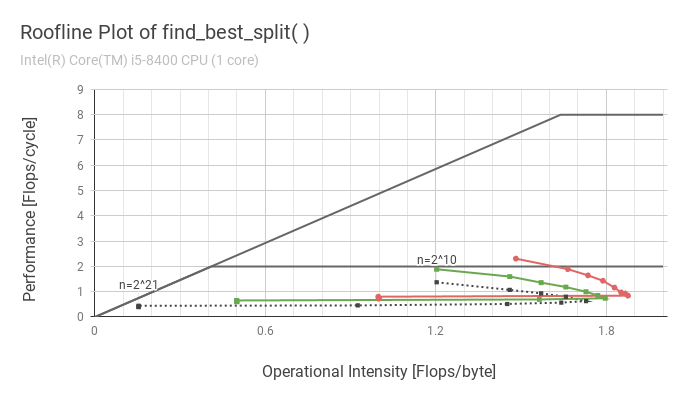
\includegraphics[width=0.47\textwidth]{fig/roofline.png}
  \caption{Roofline plot of various versions of find\_best\_split(). The baseline in black, feature\_blocking\_avx in green, feature\_blocking\_float\_avx in red.}
\end{figure}

\begin{figure}[ht]
  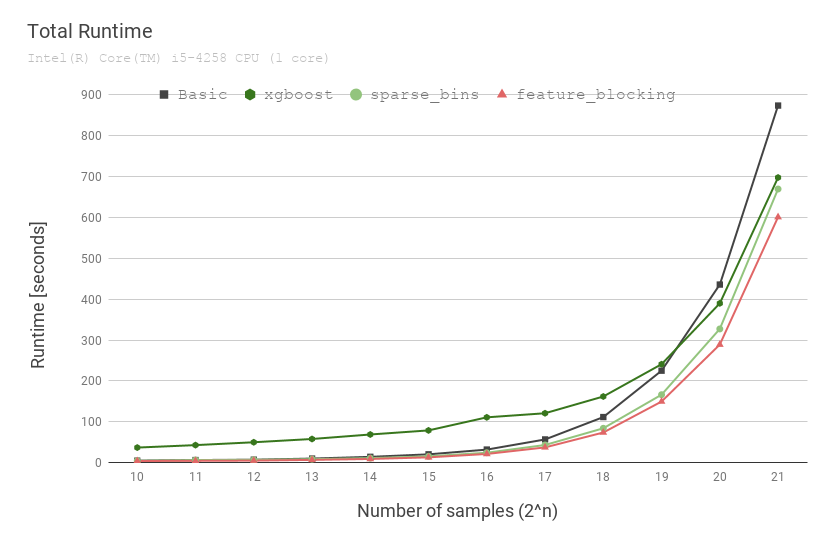
\includegraphics[width=0.47\textwidth]{fig/runtime.png}
  \caption{Runtime comparison of xgboost to our baseline, sparse bins, and feature blocking versions.}
\end{figure}